\subsection{Use Case Model}

\begin{figure}[p]
    \begin{adjustwidth}{-0.1\paperwidth}{-0.1\paperwidth}
        \centering
        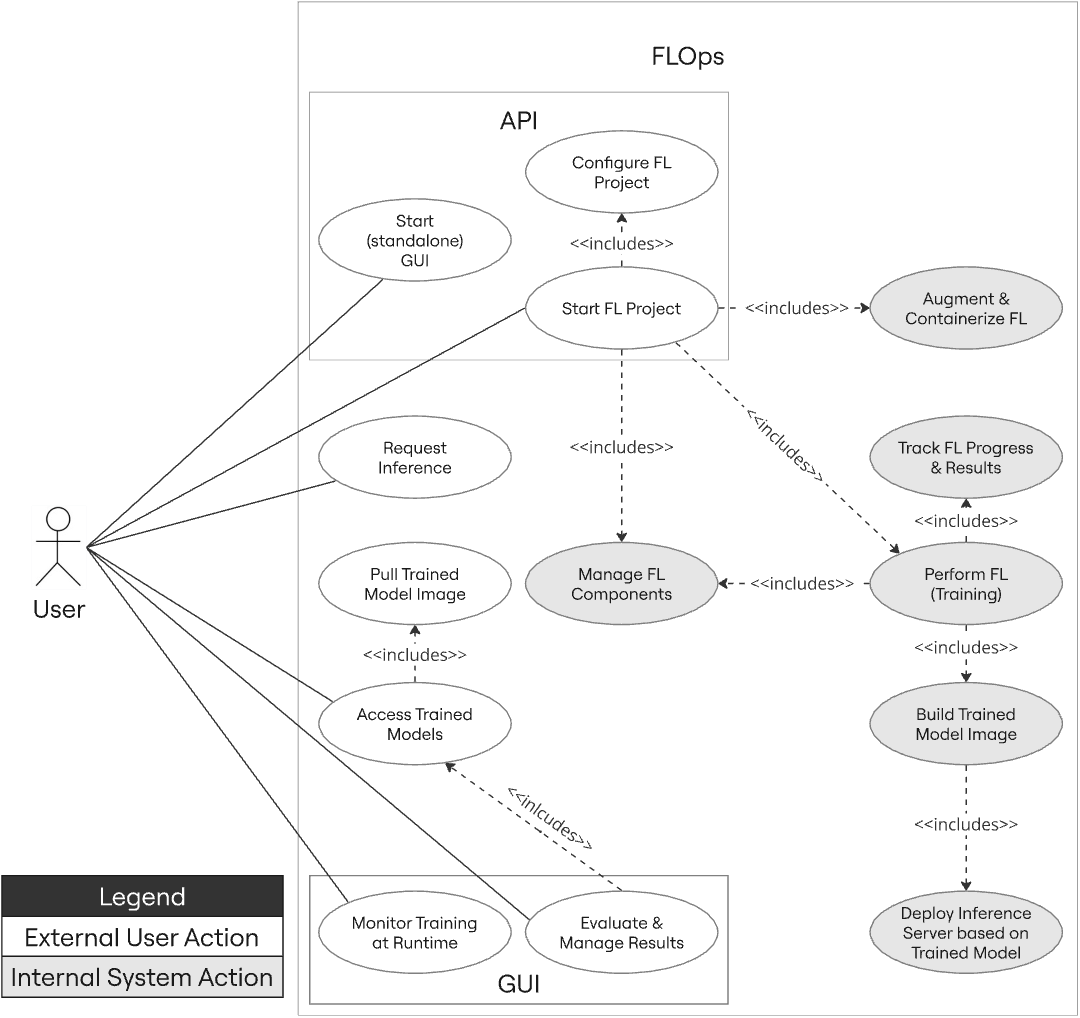
\includegraphics[width=0.9\paperwidth]{uml_use_case_diagram.png}
        \caption{FLOps UML Use Case Diagram}
        \label{fig:uml_use_case_diagram}
    \end{adjustwidth}
\end{figure}

Figure \ref{fig:uml_use_case_diagram} shows the Use Case diagram for FLOps.
The white use cases represent the functionalities the external users can directly trigger.
The grey use cases are internal system actions that are directly visible to users or lead to visible results.
They get triggered as a result of user actions.
For example, the user knows that FLOps is performing FL training by inspecting different provided outlets, such as the GUI.
FLOps tracks the training progress and results.
These logged artifacts become incrementally visible to the user who inspects the GUI.
Thus, the user knows that FLOps is currently performing FL training and logging.
Use cases inside the GUI boundary are directly accessible via the GUI. 
The same applies to the API boundary.
Other tasks are executed and accessible via FLOps combined with its orchestrator.
Use cases that involve developing or modifying FLOps itself are not explicitly portrayed.
The depicted User actor represents end users of varying FL expertise (\hyperref[FR-1.1]{FR-1.1}).
This actor includes FL developers and researchers.
The core use case is starting an FL project which also includes configuring that project (\hyperref[FR-2]{FR-2}).
This activity starts a chain of events, such as building an FL-enabled container image (\hyperref[FR-3]{FR-3}), creating and deploying the learners and aggregator(s), and performing the FL training (\hyperref[FR-1]{FR-1}).
During training, FLOps tracks the model and system metrics, which the user can monitor and evaluate in the GUI (\hyperref[FR-4]{FR-4}).
After training, the model can be containerized and deployed as an inference server (\hyperref[FR-5]{FR-5}, \hyperref[FR-6]{FR-6}).
The user can access this trained model (\hyperref[FR-5]{FR-5}) and request services from its inference server (\hyperref[FR-6]{FR-6}).
